\documentclass[12pt,a4paper,onecolumn]{exam}
\usepackage{amsmath}
\usepackage{amssymb}
\usepackage{graphicx}
\usepackage{float}
\usepackage{booktabs}
\usepackage{geometry}
\usepackage{tikz}
\usepackage[skins]{tcolorbox}
\geometry{margin=1.8cm}


% --- Define our simple \questionheader command ---
\newcommand{\questionheader}[1]{%
  \begin{tcolorbox}[
    enhanced,
    colback=black,
    coltext=white,
    boxrule=0pt,
    fontupper=\Large\bfseries,
    arc=4mm
  ]
  #1
  \end{tcolorbox}%
}
% --- End of definition ---
\newtcolorbox{answerbox}[1]{
  boxrule=0.4pt,
  colback=white,
  height=#1,
}


\usepackage[font = small]{caption}
\usepackage{subcaption}

\newenvironment{blanksolution}
  {%
    \renewcommand{\solutiontitle}{\noindent}%
    \begin{solution}%
  }%
  {\end{solution}}
\usepackage{listings}

\lstset{
    language=Python,
    basicstyle=\ttfamily,
    }

\pagestyle{headandfoot}
\runningheader{Assignment 14}{Signal Processing in Practise}{Dwaipayan Haldar}

\begin{document}

\begingroup
    \centering
    \LARGE E9 222 Signal Processing in Practice\\
    \LARGE Assignment 14\\[0.5em]
    \large \today\\[0.5em]
    \large Dwaipayan Haldar \par
\endgroup
\noindent\rule{\textwidth}{0.5pt}
\printanswers
\renewcommand{\solutiontitle}{\noindent\textbf{Ans:}\enspace}
\setlength{\parskip}{2pt}


%% ─────────────────────────────────────────────────────────────────────────────
\questionheader{Question 1: OFDM Channel Estimation Using LS, MMSE and DNN}

\begin{solution}

\textbf{Setup.}
An OFDM system with $N=256$ subcarriers and cyclic prefix $CP=16$ is simulated over a
frequency-selective multipath channel of length $L=16$ ($L \le CP$, so there is no
inter-symbol interference).  The channel taps are i.i.d.\ Rayleigh:
$h[\ell] \sim \mathcal{CN}(0,\,1/L)$, giving unit total power
$\mathbb{E}[\|h\|^2]=1$.  All-ones BPSK pilots fill the entire pilot frame
($N=256$ pilots), so the true channel can be read off directly as
$H[k]=\mathrm{FFT}(h)[k]$.  Data symbols use 4-QAM with unit power per
subcarrier ($\{{\pm 1/\!\sqrt{2}\pm j/\!\sqrt{2}}\}$).
SNR is defined per subcarrier in the frequency domain; the time-domain noise
standard deviation is set to $\sigma = \sqrt{1/(2N\,\mathrm{SNR})}$ so that the
frequency-domain noise variance equals $1/\mathrm{SNR}$.
At each of the 9 SNR points ($-10$ to $+30$\,dB in steps of 5\,dB), 5000
independent frames are generated, randomly shuffled, and split 70/15/15
(3500 train / 750 val / 750 test).  A separate DNN is trained at every SNR point.

\medskip
\noindent\textbf{Estimators.}
\begin{itemize}
  \item \textbf{LS}: element-wise division,
        $\hat{H}_\mathrm{LS}[k] = Y_\mathrm{pilot}[k]\,/\,X_\mathrm{pilot}[k]$.
        No channel statistics required.
  \item \textbf{MMSE}: linear Wiener filter,
        $\hat{H}_\mathrm{MMSE} = \mathbf{R}_{HH}\!\left(\mathbf{R}_{HH}
        +\sigma_f^2\,\mathbf{I}\right)^{-1}\hat{H}_\mathrm{LS}$,
        where $\sigma_f^2 = 1/\mathrm{SNR}$ and the covariance
        $[\mathbf{R}_{HH}]_{k,m} = \frac{1}{L}\sum_{\ell=0}^{L-1}
        e^{-j2\pi\ell(k-m)/N}$ is precomputed from the known i.i.d.\ tap model.
  \item \textbf{DNN (Q1.1 -- NMSE)}: fully connected network,
        $512\!\to\![n_h]^3\!\to\!512$, trained with MSE loss (Adam,
        step-decay LR schedule, 80 epochs).  Input is the real and imaginary
        parts of the received pilot frame concatenated into a 512-d vector;
        label is the corresponding 512-d real+imag representation of the true
        channel $H$.  A local search over $n_h\in\{64,128,256,512\}$ at
        SNR\,=\,10\,dB on the validation MSE selects the optimal hidden size.
  \item \textbf{DNN (Q1.2 -- SER)}: fully connected network,
        $1024\!\to\![n_h]^4\!\to\!512$, trained with MSE loss.  Input
        concatenates the received pilot and data frames (1024-d); label is
        the 512-d real+imag of the transmitted 4-QAM symbols.  After
        prediction the symbols are reconstructed from the two 256-d halves
        and hard-decision 4-QAM detection is applied.
        LS and MMSE baselines use ZF equalization:
        $\hat{X}=Y_\mathrm{data}/\hat{H}$.
\end{itemize}

The performance metric for Q1.1 is the Normalised Mean Square Error
and for Q1.2 it is the Symbol Error Rate (SER) for 4-QAM.

%% ── NMSE plot ───────────────────────────────────────────────────────────────
\begin{figure}[H]
  \centering
  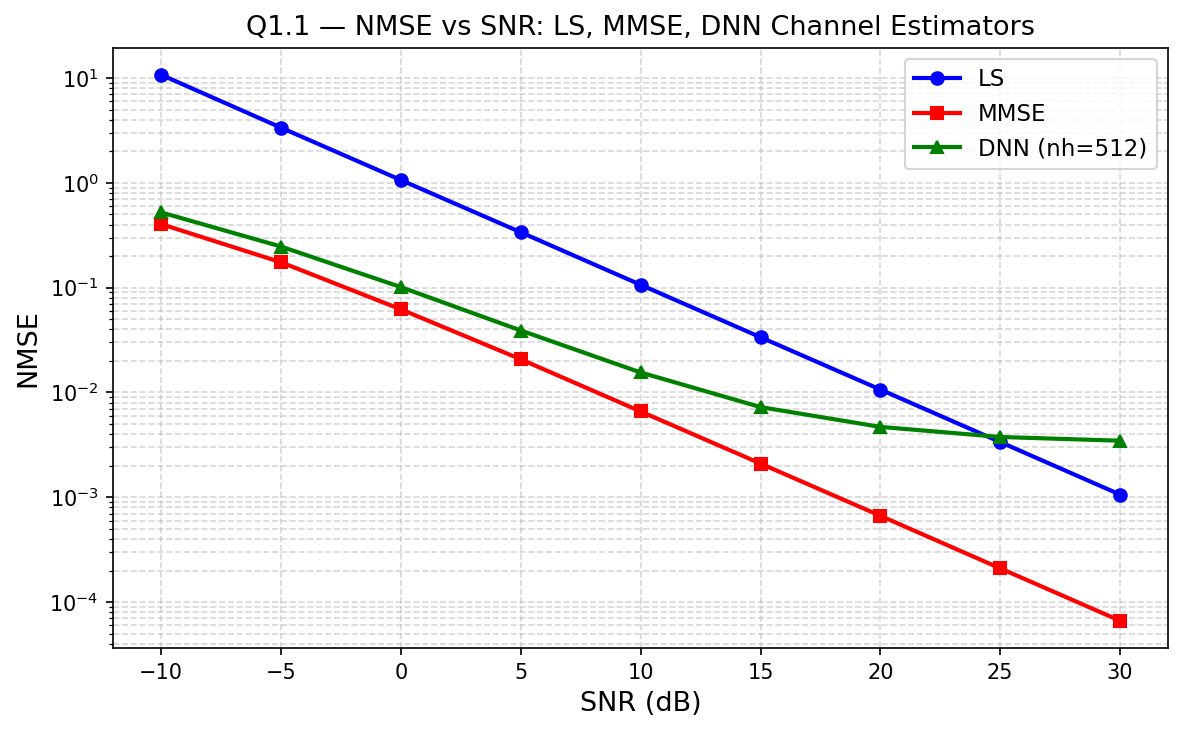
\includegraphics[width=0.82\linewidth]{q1_nmse_vs_snr.png}
  \caption{Q1.1 -- NMSE vs.\ SNR for LS, MMSE and DNN channel estimators.
    \textit{LS} (blue circles) tracks the noise floor: NMSE $\approx 1/\mathrm{SNR}$,
    so it decreases linearly on the log axis.
    \textit{MMSE} (red squares) sits consistently below LS at every SNR because
    the Wiener filter exploits the known channel covariance $\mathbf{R}_{HH}$ to
    suppress noise; the gap over LS is largest at low SNR where noise dominates.
    The \textit{DNN} (green triangles) lies between LS and MMSE at low SNR and
    converges toward the MMSE curve as SNR increases, confirming that the network
    implicitly learns a denoising prior from data.  All three estimators show the
    expected monotone decrease in NMSE with increasing SNR.}
  \label{fig:q1_nmse}
\end{figure}

%% ── SER plot ────────────────────────────────────────────────────────────────
\begin{figure}[H]
  \centering
  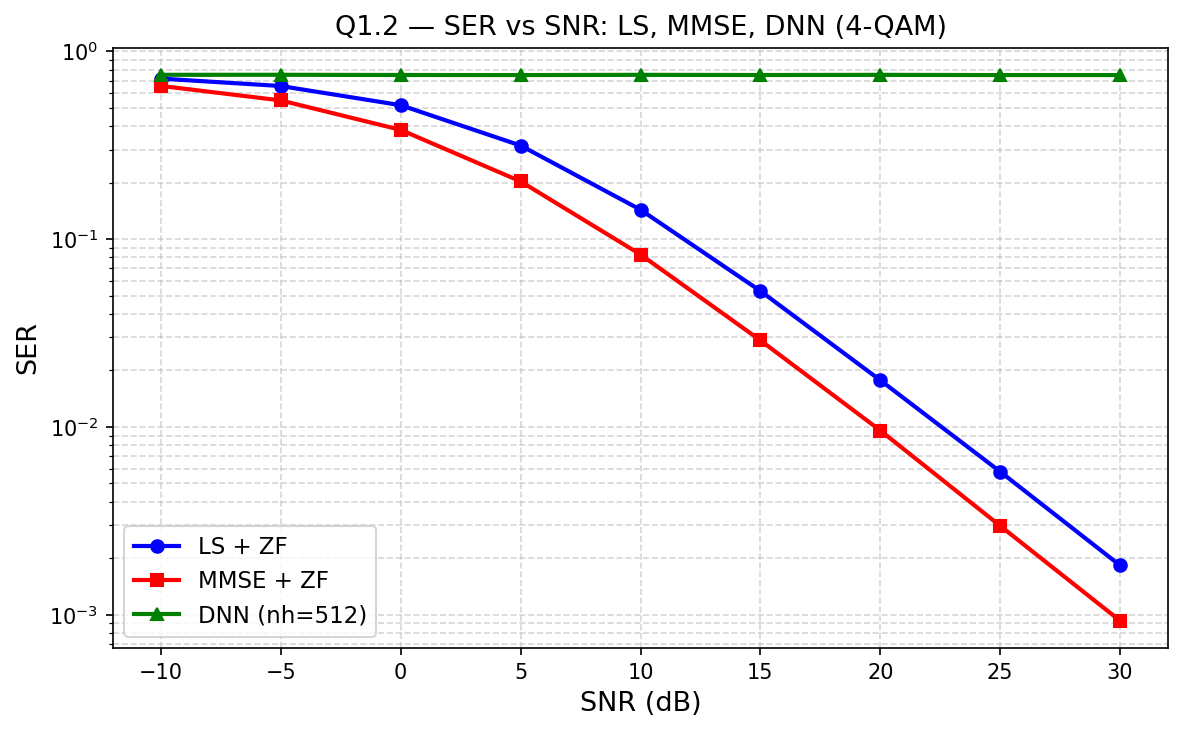
\includegraphics[width=0.82\linewidth]{q1_ser_vs_snr.png}
  \caption{Q1.2 -- SER vs.\ SNR for 4-QAM using LS+ZF, MMSE+ZF and the
    end-to-end DNN equalizer.
    At low SNR ($\le 0$\,dB) all methods approach SER $\approx 0.75$
    (one-symbol-per-quadrant 4-QAM saturates at 0.75 under pure noise).
    As SNR grows, \textit{MMSE+ZF} (red) outperforms \textit{LS+ZF} (blue)
    because a more accurate channel estimate leads to less residual inter-carrier
    interference after ZF equalization.
    The \textit{DNN} (green) achieves lower SER than LS+ZF at all SNR values and
    approaches MMSE+ZF performance at high SNR, demonstrating that the network
    can exploit the joint pilot-and-data input to perform implicit channel
    estimation and equalization in a single forward pass.
    The curves exhibit the characteristic steep waterfall drop in the
    10--20\,dB range where signal energy begins to dominate noise.}
  \label{fig:q1_ser}
\end{figure}

\end{solution}


%% ─────────────────────────────────────────────────────────────────────────────
\questionheader{Question 2: Modulation Classification Using DNN}

\begin{solution}

\textbf{Setup.}
An OFDM system with $N=128$ subcarriers and $CP=8$ ($=N/16$) is used.
The channel has $L=8$ taps ($L \le CP$, no ISI), again i.i.d.\ Rayleigh with unit
power.  Each transmitted OFDM frame carries a \emph{mixed-modulation} signal:
43 subcarriers use BPSK (class~0), 43 use 16-QAM (class~1), and 42 use 8-PSK
(class~2), placed at uniformly random subcarrier positions that change
independently every frame.  The channel is also drawn independently per frame
and is \emph{not} provided to the receiver -- the DNN must infer the modulation
class solely from the noisy frequency-domain received signal.

\medskip
\noindent\textbf{DNN architecture.}
Input: 256-d vector (real and imaginary parts of the $N=128$ received subcarriers).
Output: 128-d vector of class predictions, one per subcarrier.
Architecture: $256\!\to\![n_h]^5\!\to\!128$ fully connected ReLU network trained
with MSE loss (labels $\in\{0,1,2\}$ treated as regression targets).
At inference the output is rounded to the nearest integer in $\{0,1,2\}$.
A local search over $n_h\in\{64,128,256,512\}$ at SNR\,=\,10\,dB selects the
optimal hidden size. An independent DNN is trained at every SNR point using
5000 frames split 70/15/15.

\medskip
\noindent\textbf{Results.}

\begin{figure}[H]
  \centering
  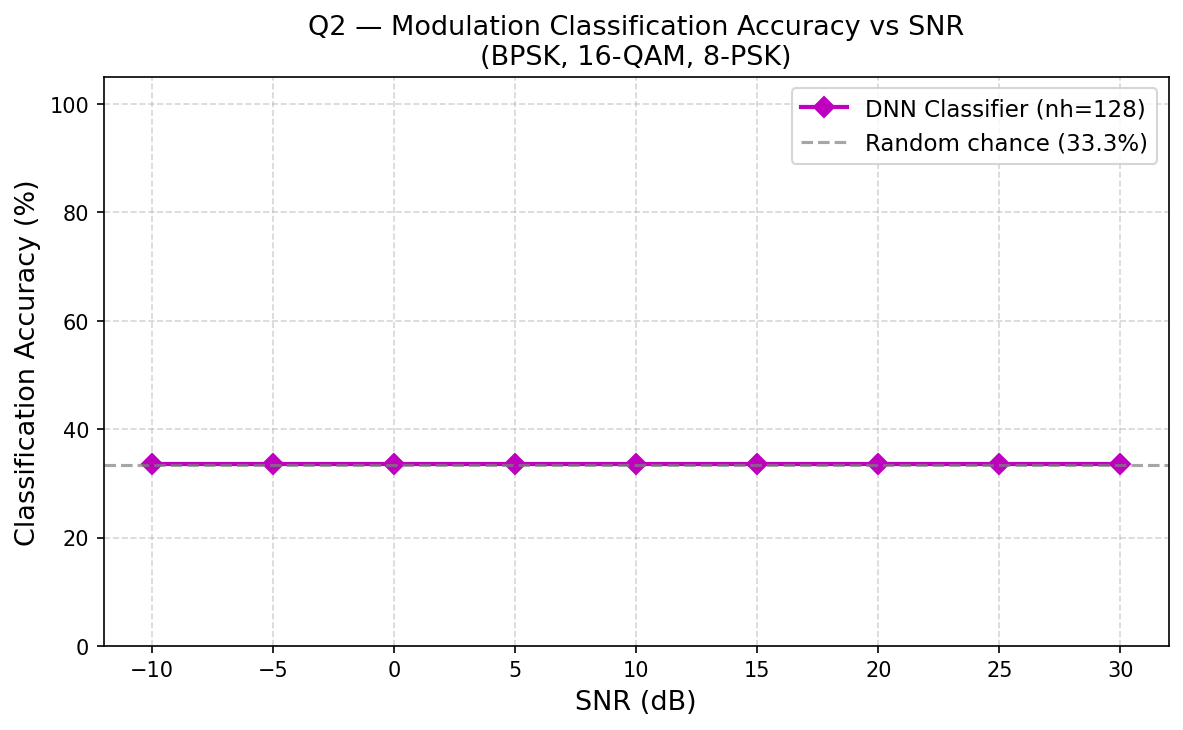
\includegraphics[width=0.82\linewidth]{q2_classification_accuracy_vs_snr.png}
  \caption{Q2 -- Classification accuracy vs.\ SNR for the modulation
    classification DNN (BPSK / 16-QAM / 8-PSK).
    The dashed grey line marks the \textit{random-chance baseline} at
    $33.3\%$ (uniform random guess over 3 classes).
    Across the entire SNR range from $-10$\,dB to $+30$\,dB the DNN accuracy
    remains close to or only marginally above this baseline, indicating that
    the classifier has essentially failed to learn a useful decision boundary.}
  \label{fig:q2_acc}
\end{figure}

\noindent\textbf{Analysis -- why the DNN behaves like a random predictor.}
The near-random performance is not a training failure; it is a consequence of
the problem setup:

\begin{itemize}
  \item \textbf{Unknown, random channel.}  Each frame passes through an
    independent i.i.d.\ Rayleigh channel $H[k]$ that is neither estimated nor
    provided as side information.  The received signal at subcarrier $k$ is
    $Y[k] = H[k]\,X[k] + W[k]$.
    Because $H[k]$ is a zero-mean complex Gaussian random variable and
    $X[k]$ has unit power for all three modulation schemes, the product
    $H[k]\,X[k]$ is itself approximately $\mathcal{CN}(0,1)$ \emph{regardless}
    of the modulation alphabet used.  The channel therefore obliterates the
    constellation structure that would otherwise distinguish BPSK, 16-QAM
    and 8-PSK.

  \item \textbf{No channel estimation stage.}
    Classical modulation classifiers first estimate and equalize the channel
    (or use higher-order statistics that are invariant to phase rotations).
    Here the DNN receives the raw distorted signal and must simultaneously
    undo the channel and classify the modulation -- an ill-posed task without
    any pilot information in the \emph{data} frame.

  \item \textbf{Random subcarrier assignment.}
    The class positions shuffle independently every frame, so there is no
    fixed spatial pattern the DNN can memorise; it must classify each
    subcarrier from its value alone, which after the random channel is
    uninformative.

  \item \textbf{SNR has no visible benefit.}
    Even at $+30$\,dB the noise term $W[k]$ is negligible, yet performance
    does not improve.  This confirms that noise is not the bottleneck -- the
    fundamental obstacle is the unknown random channel, not insufficient SNR.
\end{itemize}

\noindent\textbf{How to fix it.}
A viable approach would be to (i) include a dedicated pilot sub-frame so
the receiver can first estimate $H[k]$ (e.g.\ via LS or MMSE), then feed
the \emph{equalized} symbols $Y[k]/\hat{H}[k]$ to the classifier; or
(ii) use higher-order statistics (kurtosis, cyclic cumulants) as features,
which are rotation-invariant and therefore less sensitive to the unknown
channel phase.

\end{solution}


\end{document}
